% Lecture notes of AINIT HS26, weekend 2, Friday 14:00 and 16:00: multi-armed bandits (Once Upon a Mirror) and
% large-scale computing (computing clusters, then matrix factorization on a grid of computers). The tables and the
% figure come from generated/bandits-*.tex and generated/computing-*.tex, written by tools/afternoon_numbers.py,
% which computes every number from the games' data and checks the deck's numbers. Build: see CLAUDE.md.
\documentclass[11pt,a4paper]{article}
\usepackage[margin=2.5cm]{geometry}
\usepackage[T1]{fontenc}
\usepackage{lmodern}
\usepackage{microtype}
\usepackage{amsmath}
\usepackage{array}
\usepackage{tikz}
\usepackage{enumitem}
\usepackage{needspace}
\setlist{nosep, topsep=2pt}
\usepackage[hidelinks]{hyperref}
\urlstyle{same}
\hypersetup{pdftitle={Bandits, large-scale computing},
  pdfauthor={Carlos Cotrini}, pdfsubject={AI in Industry, ETH Zurich, weekend 2, lecture notes}}
\setlength{\parindent}{0pt}
\setlength{\parskip}{5pt plus 1pt}
\renewcommand{\arraystretch}{1.15}

\newcommand{\term}[1]{\textbf{#1}}
\newsavebox{\besidebox}
\newcommand{\beside}[2]{\par\noindent\sbox{\besidebox}{#1}\usebox{\besidebox}\hfill
  \begin{minipage}[c]{\dimexpr\textwidth-\wd\besidebox-1.5em\relax}#2\end{minipage}\par}
\newcommand{\Mirror}{\href{https://eth-ainit-hs26.github.io/AINIT-PAGE/viz/we2/mirror/}{Once Upon a Mirror}}
\newcommand{\Grid}{\href{https://eth-ainit-hs26.github.io/AINIT-PAGE/viz/we2/matchmaker-grid/}{Matchmaker on a Grid}}
\newcommand{\Clusters}{\href{https://eth-ainit-hs26.github.io/AINIT-PAGE/slides/we2/ainit-hs26-computing-clusters.pdf}{Computing clusters}}
\newcommand{\NbOne}{\href{https://colab.research.google.com/github/eth-ainit-hs26/w2-cx-public/blob/main/03_cx_bandits_1_estimates_student.ipynb}{1, the estimate}}
\newcommand{\NbTwo}{\href{https://colab.research.google.com/github/eth-ainit-hs26/w2-cx-public/blob/main/03_cx_bandits_2_random_student.ipynb}{2, the random mirror}}
\newcommand{\NbThree}{\href{https://colab.research.google.com/github/eth-ainit-hs26/w2-cx-public/blob/main/03_cx_bandits_3_estimate_then_exploit_student.ipynb}{3, estimate then exploit}}
\newcommand{\NbFour}{\href{https://colab.research.google.com/github/eth-ainit-hs26/w2-cx-public/blob/main/03_cx_bandits_4_epsilon_greedy_student.ipynb}{4, epsilon-greedy}}
\newcommand{\NbFive}{\href{https://colab.research.google.com/github/eth-ainit-hs26/w2-cx-public/blob/main/03_cx_bandits_5_ucb_student.ipynb}{5, UCB}}

\begin{document}

{\LARGE\bfseries\raggedright Bandits, large-scale computing\par}
\smallskip
Lecture notes. AI in Industry, ETH Zurich, weekend 2, Friday 13 November 2026, 14:00 and 16:00.

\section{Multi-armed bandits}

\term{Multi-armed bandit.} A series of choices among the same options. Each choice brings a reward by chance, and
only the chosen option's reward is seen. Goal: the most rewards over all the choices.

\term{The game.} Each morning a magic mirror shows its owner one ad from the Mirror Shop; a tap on the ad is a click.
A season is 100 mornings. Goal: as many taps as possible.

\term{Probability $p$.} How likely a customer is to tap a product; hidden from the mirror. Showing an ad is drawing a
ball from the customer's urn for that product, orange for a tap: Cinderella's urn for the mattress holds 2 orange
balls of 5, $p = 2/5 = 0.4$.
\begin{center}
% GENERATED by tools/afternoon_numbers.py: do not edit, run the script.
\begin{tabular}{|l|c|c|c|c|c|}
\hline
 & Robot vacuum & Rope ladder & Leaf blower & Memory-foam mattress & Satnav \\ \hline
Cinderella & $0.6$ & $0.2$ & $0.2$ & $0.4$ & $0.2$ \\ \hline
Rapunzel & $0.4$ & $0.8$ & $0.2$ & $0.2$ & $0.2$ \\ \hline
\end{tabular}

\end{center}

\term{Estimate $\hat p$.} Of a product: its taps divided by its showings, the average of its 1s (taps) and 0s (no
taps). The more showings, the closer it tends to get to $p$. The board has one row per product and one dot per
showing: $\bullet$ a tap, $\circ$ no tap.

\term{Rate.} Of a season: taps divided by mornings. The rate so far, after each morning: the taps so far divided by
the mornings so far.

\term{The Queen's mirror.} It knows every $p$ and shows the product with the highest $p$ every morning: an imagined
reference, the best rate a mirror could reach.

\term{Strategy.} The rule a mirror follows to choose the ad each morning, from the dots alone. To initialize is to show
each product once, in the order of the board, on mornings 1 to 5.

\term{Exploration-exploitation dilemma.} Each morning the mirror explores, showing a product to learn more about it,
or exploits, showing the product with the highest estimate. Explore too little and it may never find the favourite.
Explore too much and it wastes mornings.

Game: \Mirror, section 1. Notebook: \NbOne.

\section{Random}

\term{Random.} Each morning, a card from a hat: every product has the same chance, 1 in 5. Random never looks at the
estimates.

\term{Race season.} The season on which the game plays every mirror: the same mornings, the same Cinderella.
Random: 31 taps, rate $0.31$. The Queen's mirror, the vacuum every morning: 60 taps, rate $0.6$.

Game: \Mirror, section 2. Notebook: \NbTwo.

\section{Estimate then exploit}

\term{Estimate then exploit} with $n$:
\begin{enumerate}
\item Initialize.
\item Test: on each of the next $n$ mornings, a card from the hat.
\item Highest estimate: after the test, the product with the highest estimate; a tie is broken at random.
\item Exploit: show it on every remaining morning.
\end{enumerate}

\needspace{7\baselineskip}
\beside{% GENERATED by tools/afternoon_numbers.py: do not edit, run the script.
\begin{tabular}{|c|c|l|l|}
\hline
$\hat p$ & & Product & Showings \\ \hline
$0.67$ & $2/3$ & Robot vacuum & $\circ$\,$\bullet$\,$\bullet$ \\ \hline
$0$ & $0/4$ & Rope ladder & $\circ$\,$\circ$\,$\circ$\,$\circ$ \\ \hline
$0$ & $0/5$ & Leaf blower & $\circ$\,$\circ$\,$\circ$\,$\circ$\,$\circ$ \\ \hline
$0.38$ & $3/8$ & Memory-foam mattress & $\bullet$\,$\circ$\,$\circ$\,$\bullet$\,$\bullet$\,$\circ$\,$\circ$\,$\circ$ \\ \hline
$0.2$ & $1/5$ & Satnav & $\circ$\,$\circ$\,$\circ$\,$\circ$\,$\bullet$ \\ \hline
\end{tabular}
}{Example: the race season with $n = 20$, the board after the test,
mornings 1 to 25. The vacuum leads with $0.67$; the mirror shows it on mornings 26 to 100. Taps: 6 in the test, 41
after, 47 in all.}

\term{Choosing $n$.} A large $n$ wastes mornings on products the customer rarely taps; with a small $n$, a weaker
product can have the highest estimate. The best $n$ depends on the probabilities, which the mirror does not know.
The challenge round, the average rate over 10,000 seasons for every $n$ from 0 to 95, the best $n$ within $0.005$ of
the highest: Ready for the ball, Cinderella (silk gloves 0.6, tiara 0.9, evening bag 0.6, ball gown 0.95, lipstick
0.6), best $n$ 19 to 34; Long hair, Rapunzel (ribbon 0.95; scissors, cap, razor and haircut voucher 0.02 each), best
$n$ 1 to 6.

Game: \Mirror, section 3. Notebook: \NbThree.

\section{Epsilon-greedy}

\term{Epsilon-greedy} with $\varepsilon$, the share of the roulette's small slice:
\begin{enumerate}
\item Initialize.
\item Spin the roulette. With $\varepsilon = 0.2$, one spin in five stops on the small slice.
\item Sample: on the small slice, a card from the hat, every product with the same chance, the best one too; on the
  large slice, the product with the highest estimate, a tie broken at random.
\item Update: tap or no tap, the estimate of the product shown changes. Steps 2 to 4 repeat every morning.
\end{enumerate}

Example: the race season with $\varepsilon = 0.2$. The needle stopped on the hat 16 times in 95 spins. From morning
19 on, the large slice always showed the vacuum. Showings in the season: vacuum 71, ladder 6, blower 2, mattress 16,
satnav 5. Taps: 47.

Game: \Mirror, section 4. Notebook: \NbFour.

\section{UCB}

\term{Exploration bonus.} Of a product with $n$ dots: $1/\sqrt{n}$. The fewer dots, the bigger the bonus.

\term{UCB.} Upper confidence bound:
\begin{enumerate}
\item Initialize: each product's first estimate and first bonus.
\item Show the highest: the product with the highest estimate + bonus; a tie is broken at random.
\item Update: tap or no tap, its estimate and its bonus change.
\item Repeat every morning, to the end of the season.
\end{enumerate}

\needspace{9\baselineskip}
Example: the race season after 10 mornings; in the game the estimate is the dark bar, the bonus the light bar.
\begin{center}
% GENERATED by tools/afternoon_numbers.py: do not edit, run the script.
\begin{tabular}{|l|l|c|c|c|}
\hline
Product & Showings & Estimate & Bonus & Estimate + bonus \\ \hline
Robot vacuum & $\circ$\,$\bullet$\,$\bullet$\,$\bullet$ & $3/4 = 0.75$ & $1/\sqrt{4} = 0.5$ & $1.25$ \\ \hline
Rope ladder & $\circ$ & $0/1 = 0$ & $1/\sqrt{1} = 1$ & $1$ \\ \hline
Leaf blower & $\circ$ & $0/1 = 0$ & $1/\sqrt{1} = 1$ & $1$ \\ \hline
Memory-foam mattress & $\bullet$\,$\circ$\,$\circ$ & $1/3 = 0.33$ & $1/\sqrt{3} = 0.58$ & $0.91$ \\ \hline
Satnav & $\circ$ & $0/1 = 0$ & $1/\sqrt{1} = 1$ & $1$ \\ \hline
\end{tabular}

\end{center}
The highest estimate + bonus: the vacuum, 1.25. The mirror shows it on morning 11. Taps in the season: 52.

\term{The real UCB.} The product with the highest $\hat p + \sqrt{2 \ln t / n}$, $t$ the mornings so far, $\ln$ the
natural logarithm. With high confidence, $p$ is below this number: an upper confidence bound. Its bonus grows slowly
with $t$, so a product left aside long enough comes back. The game's bonus $1/\sqrt{n}$ leaves $t$ out.

\needspace{7\baselineskip}
\term{All the mirrors.}
\beside{% GENERATED by tools/afternoon_numbers.py: do not edit, run the script.
\begin{tabular}{|l|c|c|}
\hline
Mirror & Cinderella & Rapunzel \\ \hline
Queen's mirror & 60 & 78 \\ \hline
UCB & 52 & 70 \\ \hline
Epsilon-greedy, $\varepsilon = 0.2$ & 47 & 67 \\ \hline
Estimate then exploit, $n = 20$ & 47 & 61 \\ \hline
Random & 31 & 32 \\ \hline
\end{tabular}
}{Taps in the race season, every mirror on the same 100 mornings. At
Rapunzel's the ladder, $p = 0.8$, stands far above her other products. Another season gives other numbers.}

Game: \Mirror, section 5. Notebook: \NbFive.

\section{Computing clusters}

\term{FLOP.} Floating point operation: one operation, such as a multiply or an add, on two numbers; $a \times b + c$
is 2 FLOPs. FLOPs count work; FLOP/s, operations per second, measure speed.

\term{GH200.} A module of NVIDIA: Grace, an ARM CPU, and Hopper, the GPU that does the arithmetic, with 96 GB of
HBM3 memory. Rate: $990 \times 10^{12}$ FLOP/s at 16 bits per number. A human computer of 1949: 1,000 additions a
day.

\term{Socket and node.} A socket is one processor module, here one GH200. A node is one independent computer, here 4
GH200 with one operating system and one address space.

\term{Alps.} The machine of CSCS, the Swiss National Supercomputing Centre in Lugano, an HPE Cray EX254n: 24 cabinets
of 8 chassis, 7 blades in each chassis, 2 nodes on each blade. 2,688 nodes $\times$ 4 GH200 $=$ 10,752 sockets,
$10.6 \times 10^{18}$ FLOP/s together. Apertus, the open language model of EPFL, ETH Zurich and CSCS, was
trained on Alps.

\term{Capacity and bandwidth.} Capacity: how much fits, 96 GB on a GH200. Bandwidth: how fast it moves, 4 TB/s from
the HBM3 memory. $990 \times 10^{12}$ FLOP/s divided by $4.023 \times 10^{12}$ bytes/s is 246 FLOP per byte: unless a
computation reuses each byte about that many times, the arithmetic units wait. A large matrix multiply does; many
other operations do not.

\term{Links.} The GPU to its HBM3 memory, 4,023 GB/s; Grace to Hopper, 900 GB/s; socket to socket inside a node,
150 GB/s; between nodes, 25 GB/s per GPU. Each step down costs about a factor of five; end to end, 161 times. The
data stays at the fast end, and the slow links are crossed as rarely as possible.

\term{Watt and kilowatt hour.} A watt is a rate of energy, a kilowatt hour an amount: rate $\times$ time $=$ amount,
as FLOP/s $\times$ seconds $=$ FLOP. Alps caps each GH200 at about 660 W: one hour takes 0.66 kWh, 5.3 Rappen at 8
Rappen per kWh (assumed). All 10,752 modules: 7.1 MW, about 570 francs an hour.

\term{Training cost.} $C = 6ND$ FLOP for a model of $N$ parameters trained on $D$ training numbers; the 6 is a rule
of thumb. $N = D = 10^6$: $C = 6 \times 10^{12}$ FLOP, 120 seconds on a laptop at $50 \times 10^9$ FLOP/s.
Apertus-70B, $N = 70 \times 10^9$, $D = 15 \times 10^{12}$: $C = 6.30 \times 10^{24}$ FLOP.

\term{The Apertus-70B run.} Over 6 million GPU hours on up to 4,096 GPUs: 61 days of 4,096 GPUs flat out. The run
spanned about 91 days, 2,747 GPUs on average. Energy: 6 million GPU hours $\times$ 660 W $=$ 3.96 GWh, 0.32 million
francs at 8 Rappen per kWh. At a cloud rate of \$2.50 per GPU hour: \$15.0 million.

Slides: \Clusters.

\section{Matrix factorization on a grid of computers}

\term{The job.} \Grid: 6 customers and 6 films, two guessed numbers each. Gradient descent keeps 132 numbers: 36
ratings, 24 guessed numbers (12 of the customers, 12 of the films), 36 predictions and 36 losses. Each of 15
computers has room for 21 numbers: neither the ratings (36) nor the guessed numbers (24) fit in one, and together the
computers have 315 places.

\term{Blocks and slices.} The 4 predictions of 2 customers and 2 films need only the two rows of those customers and
the two columns of those films, 8 of the 24 guessed numbers. The ratings, cut every 2 customers and every 2 films:
nine blocks of 4 ratings, one on each of the computers C11 to C33. The customers' numbers, cut into 3 slices of 2
customers: A1 to A3. The films' numbers, cut into 3 slices of 2 films: B1 to B3. A C computer holds 4 ratings, 4 + 4
copies, 4 predictions, 4 losses and their sum: 21 numbers.

\needspace{12\baselineskip}
\begin{center}
% GENERATED by tools/afternoon_numbers.py: do not edit, run the script.
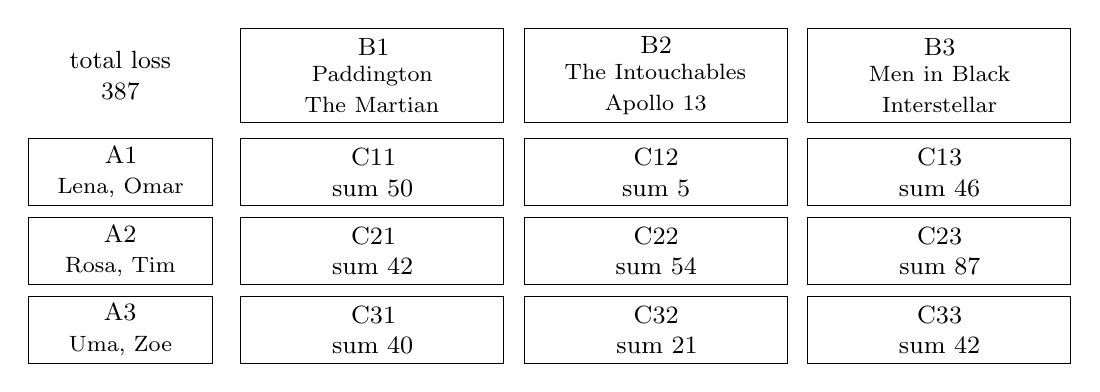
\begin{tikzpicture}[x=1cm, y=1cm, every node/.style={font=\small, align=center, inner sep=2pt}]
\node[draw, text width=3.20cm, minimum height=1.20cm] at (4.40, 0) {B1\\ {\footnotesize Paddington\\ The Martian}};
\node[draw, text width=3.20cm, minimum height=1.20cm] at (8.00, 0) {B2\\ {\footnotesize The Intouchables\\ Apollo 13}};
\node[draw, text width=3.20cm, minimum height=1.20cm] at (11.60, 0) {B3\\ {\footnotesize Men in Black\\ Interstellar}};
\node[draw, text width=2.20cm, minimum height=0.85cm] at (1.20, -1.23) {A1\\ {\footnotesize Lena, Omar}};
\node[draw, text width=3.20cm, minimum height=0.85cm] at (4.40, -1.23) {C11\\ sum 50};
\node[draw, text width=3.20cm, minimum height=0.85cm] at (8.00, -1.23) {C12\\ sum 5};
\node[draw, text width=3.20cm, minimum height=0.85cm] at (11.60, -1.23) {C13\\ sum 46};
\node[draw, text width=2.20cm, minimum height=0.85cm] at (1.20, -2.23) {A2\\ {\footnotesize Rosa, Tim}};
\node[draw, text width=3.20cm, minimum height=0.85cm] at (4.40, -2.23) {C21\\ sum 42};
\node[draw, text width=3.20cm, minimum height=0.85cm] at (8.00, -2.23) {C22\\ sum 54};
\node[draw, text width=3.20cm, minimum height=0.85cm] at (11.60, -2.23) {C23\\ sum 87};
\node[draw, text width=2.20cm, minimum height=0.85cm] at (1.20, -3.23) {A3\\ {\footnotesize Uma, Zoe}};
\node[draw, text width=3.20cm, minimum height=0.85cm] at (4.40, -3.23) {C31\\ sum 40};
\node[draw, text width=3.20cm, minimum height=0.85cm] at (8.00, -3.23) {C32\\ sum 21};
\node[draw, text width=3.20cm, minimum height=0.85cm] at (11.60, -3.23) {C33\\ sum 42};
\node at (1.20, 0) {total loss\\ 387};
\end{tikzpicture}

\end{center}

\term{Gradient descent on the grid.}
\begin{enumerate}
\item Every A computer sends a copy of its numbers to the 3 C computers of its row.
\item Every B computer sends a copy of its numbers to the 3 C computers of its column.
\item Every C computer multiplies its two copies: its 4 predictions.
\item Every C computer computes its 4 losses and their sum. The nine sums add up to the total loss.
\item What-if: one number of an A or B computer changes by 0.01. Only the C computers of its row or column use it;
  they recompute their sums, and the nine sums give the total loss after.
\item Slope: (total loss after $-$ total loss before)$/0.01$.
\item Update: the number moves to number $- \alpha \times$ slope, with $\alpha = 0.014$.
\item Rounds: every number of A and B does its what-if at the same guess, then all move at once.
\end{enumerate}

Example: the first guess, above, has total loss 387. The Intouchables' first number, on B2, from $-1$ to $-0.99$:
only C12, C22 and C32 recompute, their sums 5 to 4.9005, 54 to 53.8005 and 21 to 21.0405, and the total loss goes
from 387 to 386.7415. Slope: $(386.7415 - 387)/0.01 = -25.85$. Update: $-1 - 0.014 \times (-25.85) = -0.64$. The
total loss is below 1 after round 30 and below 0.01 after round 51; it stops falling after round 78, at 0.0028, every
prediction within 0.022 of its rating.

Game: \Grid.

\section{Games, notebooks and slides}

Game, visualization and slides, on the course site:

{\small
\begin{tabular}{@{}l@{\hspace{0.6em}}l@{}}
Once Upon a Mirror & {\scriptsize\url{https://eth-ainit-hs26.github.io/AINIT-PAGE/viz/we2/mirror/}} \\
Matchmaker on a Grid & {\scriptsize\url{https://eth-ainit-hs26.github.io/AINIT-PAGE/viz/we2/matchmaker-grid/}} \\
Computing clusters & {\scriptsize\url{https://eth-ainit-hs26.github.io/AINIT-PAGE/slides/we2/ainit-hs26-computing-clusters.pdf}} \\
\end{tabular}\par}

Notebooks, in the public repository \url{https://github.com/eth-ainit-hs26/w2-cx-public}. Each link opens a
notebook in Colab:

{\small
\begin{tabular}{@{}l@{\hspace{1.2em}}l@{}}
1, the estimate & \href{https://colab.research.google.com/github/eth-ainit-hs26/w2-cx-public/blob/main/03_cx_bandits_1_estimates_student.ipynb}{student}, \href{https://colab.research.google.com/github/eth-ainit-hs26/w2-cx-public/blob/main/03_cx_bandits_1_estimates_solutions.ipynb}{solutions} \\
2, the random mirror & \href{https://colab.research.google.com/github/eth-ainit-hs26/w2-cx-public/blob/main/03_cx_bandits_2_random_student.ipynb}{student}, \href{https://colab.research.google.com/github/eth-ainit-hs26/w2-cx-public/blob/main/03_cx_bandits_2_random_solutions.ipynb}{solutions} \\
3, estimate then exploit & \href{https://colab.research.google.com/github/eth-ainit-hs26/w2-cx-public/blob/main/03_cx_bandits_3_estimate_then_exploit_student.ipynb}{student}, \href{https://colab.research.google.com/github/eth-ainit-hs26/w2-cx-public/blob/main/03_cx_bandits_3_estimate_then_exploit_solutions.ipynb}{solutions} \\
4, epsilon-greedy & \href{https://colab.research.google.com/github/eth-ainit-hs26/w2-cx-public/blob/main/03_cx_bandits_4_epsilon_greedy_student.ipynb}{student}, \href{https://colab.research.google.com/github/eth-ainit-hs26/w2-cx-public/blob/main/03_cx_bandits_4_epsilon_greedy_solutions.ipynb}{solutions} \\
5, UCB & \href{https://colab.research.google.com/github/eth-ainit-hs26/w2-cx-public/blob/main/03_cx_bandits_5_ucb_student.ipynb}{student}, \href{https://colab.research.google.com/github/eth-ainit-hs26/w2-cx-public/blob/main/03_cx_bandits_5_ucb_solutions.ipynb}{solutions} \\
\end{tabular}\par}

\end{document}
